\chapter{Methodologies}
\label{chap:methods}

This chapter illustrates the methodology used to approach the development process of this work.The application is divided into three main independent instances: gesture recognition, 3D trajectory detection and drone controller. First of all, the Section \ref{sec:handgestrec} to create a \gls{dnn} model to recognize hand gestures, followed by Section \ref{sec:getdata} and \ref{sec:model} that describes the type of data used for this purpose and how they are generated. After, we will see about how orientation and camera-hand distance has been estimated in Section \ref{sec:orientationestimation} and \ref{subsec:cam-hand} to detect a 3D trajectory. Next, we focus on the drone controller in simulation and real. We conclude Section \ref{sec:pipeline} with a detailed explanation of the entire pipeline.

%pipeline
%mediapipe (poco perché già parlato tecnicamente)
%costruzione della rete neurale:
%	come devono essere i dati
%trasformazione matriciale
%algoritmo dei tre punti orientamento
%pitch
%yaw
%roll

\section{Hand Gesture Recognition}
\label{sec:handgestrec}
MediaPipe has a python implementation for their Hand Keypoints Detector. It returns 2.5D coordinates of 21 hand landmarks (see Fig.\ref{fig:handland}), consisting of $x$, $y$, and relative $depth$. For this project the $depth$ coordinate of each hand landmark have been deleted because we wanted to estimate them.

% https://towardsdatascience.com/control-dji-tello-drone-with-hand-gestures-b76bd1d4644f

\begin{figure}[H]
	\centering
	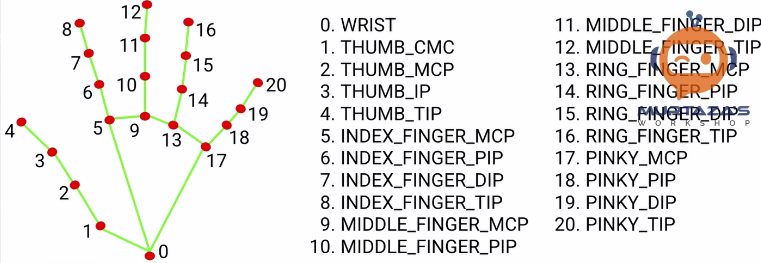
\includegraphics[width=.9\textwidth]{images/hand}
	\caption[Hand Landmarks.]{Image from the open MediaPipe repository.}
	\label{fig:handland}
\end{figure}

\noindent The coordinates of pixels in OpenCV follow a reference system $(x,y)$ in which the origin is in top-left of each image frame, $x$ is column-wise and $y$ is row-wise on the computer screen. In order to normalize each point, the origin has been converted from top-left to bottom-left. This gives us the classic cartesian coordinate system. After, for each landmark has been computed the mean for $x$ and $y$, converted in homogeneous coordinates and shifted them in order to match mean with origin. Note that shifting the data did not change how the data points are positioned relative to each other. Finally, each point has been scaled respect the max distance from mean point to all other hand points. This normalization permits to compare same gesture at different distance from camera, if same orientation. 

\subsection{Data Acquisition and Description}
\label{sec:getdata}
Following the normalization of the data, it was thought of gestures that would allow firstly to acquire a 3D trajectory and secondly to interact directly with the drone. \\

\begin{figure}[H]
	\centering
	\includegraphics[width=1 \textwidth]{images/gestures}
	\caption[Full list of gestures.]{Full list of gestures that are available.}
	\label{fig:gestures}
\end{figure}

\noindent Below is the list of 10 gestures used in our project:
\begin{itemize}
	\item \texttt{backward}: this command allows the drone to go backwards;
	\item \texttt{detect}: this command allows you to detect a \gls{3d} trajectory;
	\item \texttt{down}: this command allows the drone to go down;
	\item \texttt{forward}: this command allows the drone to go forward;
	\item \texttt{land}: this command allows the drone to land;
	\item \texttt{left}: this command allows the drone to go left;
	\item \texttt{ok}: this command allows the drone to go close and execute a \gls{3d} trajectory;
	\item \texttt{right}: this command allows the drone to go right;
	\item \texttt{stop}: this command allows the drone to stop his movements;
	\item \texttt{up}: this command allows the drone to go up.
\end{itemize}

\noindent From the module that has been built is there the possibility to get data either from a webcam or from the drone camera. The dataset consists of $42000$ elements because $100$ images are acquired for each gesture and each gesture has $21$ points $(x,y)$. The python script to get data has also a restore in case of particular error (for example if images are acquired from the drone could be problems due to overheating or low battery). Given the structure of the generation script it is particularly easy to build a model with new gestures.

\subsection{Model}
\label{sec:model}
Now we are ready to choose a model. For classification tasks there are variety of different estimators/models that we can pick from. In the end, DNNClassifier was chosen. We built a \gls{dnn} with two hidden layers with $30$ and $10$ nodes each. Input layer is composed of 42 elements and the output layer of 10 classes (see Fig. \ref{fig:handarch}). The model must choose among ten classes. The activation function is the Leaky ReLU and Adam the optimizer with learning rate $0.1$, decay steps $10000$ and decay rate $0.96$. About steps for the training phase has been chosen $3000$ as value. Loss is calculated by using softmax cross entropy.

% https://github.com/ashishpatel26/Tools-to-Design-or-Visualize-Architecture-of-Neural-Network
% http://alexlenail.me/NN-SVG/index.html
\begin{figure}[H]
	\begin{minipage}{\textwidth}
		\centering
		\includegraphics[width=1 \textwidth]{images/net}
		\caption[Hand gesture reconognition \gls{nn}.] {\gls{nn} image of the hand gesture recognition, generated by NNSVG\footnote{\url{http://alexlenail.me/NN-SVG/index.html}}.}
		\label{fig:handarch}
	\end{minipage}
\end{figure}

\noindent Because of such a simple structure,  high accuracy with a small number of examples was reached. It is not required to retrain the model for each gesture in different illumination, because MediaPipe takes over all the detection work.

\section{3D trajectory detection}
\label{sec:3dtraj}
Trajectories will be detected using the detect gesture (see Fig. \ref{fig:gestures} (c)). The experiments about orientation estimation will be executed just only on that gesture. 

\subsection{Orientation estimation}
\label{sec:orientationestimation}
In the following section, we will discuss the methods used to perform yaw, roll and pitch measurements starting from the pixels of the image captured with a camera.

\subsubsection{Turning and orientations}
\label{subsec:orientationtest}
%ATTENZIONE DA FARE (citare cmsc754-spring2020-lects)
In order to find a value for the yaw we need to understand how to determine whether three points form a left-hand turn. This can be done by an orientation test, which is fundamental to many algorithms in computational geometry (citare cmsc754-spring2020-lects). Given an ordered triple of points $\langle p, q, r \rangle$ in the plane, we say that they have positive orientation if they define a counterclockwise oriented triangle (see Fig. \ref{fig:orientationtest} (a)), negative orientation if they define a clockwise oriented triangle (see Fig. \ref{fig:orientationtest} (b)), and zero orientation if they are collinear, which includes as well the case where two or more of the points are identical (see Fig. \ref{fig:orientationtest} (c)). It is important take care about the fact that the orientation depends on the order in which the points are given.

\begin{figure}[H]
	\centering
	\includegraphics[width=.8\textwidth]{images/orientationtest}
	\caption[Orientation test.]{Orientations of the ordered triple (p, q, r).}
	\label{fig:orientationtest}
\end{figure}

\noindent Orientation is formally defined as the sign of the determinant of the points given in homogeneous coordinates, that is, by prepending a 1 to each coordinate. For example, in the plane, we define:

% https://jasonwarta.github.io/latex-matrix/ 
\begin{Equation}[!htb]
	\centering
	\begin{equation} \label{eq:orientationtest}
		Orient(p,q,r) = det
		\begin{pmatrix}
		1 & p_x & p_y \\
		1 & q_x & q_y \\
		1 & r_x & r_y 
		\end{pmatrix}
		\end{equation}
	\caption[Orientation test.]{Thus orientation generalizes the familiar 1-dimensional binary relations $<, =, >$.}
\end{Equation}

\noindent The sign of the orientation of an ordered triple is unchanged if the points are translated, rotated, or scaled (by a positive scale factor). In general, applying any affine transformation to the point alters the sign of the orientation according to the sign of the determinant of the matrix used in the transformation. \\

\noindent If we consider points belonging to the same reference system and compute the orientation test then we can get information of how much the points are crushed together. 

\subsubsection{Roll estimation}
\label{subsec:roll}
To estimate the roll, we found the angle generated by the vertical axis passing over the wrist and the tip of the middle finger (see fig. \ref{fig:handland}).

\subsubsection{Yaw estimation}
\label{subsec:yaw}
First of all, to estimate the yaw, it is necessary to fix a hand. This project will be on the left-hand, so each comment will be in that direction. Despite this, the same can be said for the right hand. Then, we compute the orientation test (see Eq. \ref{eq:orientationtest}) of three points $\langle p, q, r \rangle$. As already said, the order here is important to find the direction of orientation, therefore to know if the left-hand points left or right and with which intensity. We have seen empirically that if $roll < \ang{-5}$ or $roll > \ang{+5}$ it is better to consider $p=$ index\_finger\_mcp, $q=$ index\_finger\_pip and $r=$ index\_finger\_dip. Otherwise, if $\ang{-5} < roll < \ang{+5}$ we have noted that good results if $p=$ middle\_finger\_mcp, $q=$ middle\_finger\_pip and $r=$ middle\_finger\_dip. These hand points were chosen because they scale quite well with hand orientation. \\

\noindent The value of the orientation test is elevated to the second power, in order to be more stable around \ang{0}. Then, it is divided by $1666$, a value computed empirically to bring the results obtained from the orientation test to the range of \ang{-90} to \ang{+90}. Since we used the quadratic form, this value will be very huge if greater than \ang{+90} or smaller than \ang{-90}, for this reason the part the exceeds has been reduced to be just the $10\%$ of it.

\subsubsection{Pitch estimation}
\label{subsec:pitch}
To compute pitch estimation, we compute the middle point $m$ between index\_finger\_mcp and index\_finger\_pip and then the difference between $m$ and the thumb\_tip, respect vertical axis (see fig. \ref{fig:handland}). Also here, as for yaw estimation, the value obtained is elevated to the second power, in order to be more stable around \ang{0}. Then, we divided the result by $31$ (empirically computed), to bring the results to the range of \ang{-90} to \ang{90}. Since we used the quadratic form, also here if the value is greater than \ang{90} or smaller than \ang{-90} the results tends to be really big, therefore the part the exceeds has been reduced to be just the 10\% of it.

\subsection{Camera-hand distance estimation}
\label{subsec:cam-hand}

\subsection{Univariate spline}
\label{sec:univspline}
Fitting data

\section{Drone controller}
\label{sec:dronecontrl}

\subsection{Simulation}
\label{sec:simulation}

\subsection{Real world}
\label{sec:simulation}

\section{Pipeline}
\label{sec:pipeline}
